%=========================================================================
% (c) Michal Bidlo, Bohuslav Křena, 2008


%čo všetko môžem prebrať z BP?
%graf s num. chybami? nie
%čo všetko môžem prebrať zo závadovej BP?priloha
%čo všetko môžem prebrať od čambora? popis násobenia/sčítania priloha
%na kolko členov bude pracovať taylorová rada? treba tolko registrov 20/40
%aká sústava rovníc? aké zapojenie?
%ako bude prebiehať obhajoba?
%pevná rádová čiarka obrázok je česky....mám rperobiť na slovenský?netreba

\chapter{Úvod}
Hlavným cieľom tejto práce je návrh harvérových komponentov na riešenie rozsiahlych diferenciálnych rovníc. Diferenciálne rovnice sa väčšinou riešia pomocou numerickej integrácie, a teda s~použitím vhodných numerických metód. Hardvérový komponent využívajúci numerickú integráciu sa nazýva numerický integrátor.

V~kapitole~\ref{NUM_INTEGRACIA} sú predstavené rôzne numerické metódy - Eulerova metóda, metóda Runge-Kutta a Taylorov rad. Najväčšia pozornosť je venovaná metóde Taylorovej rady, ktorá poskytuje vhodný pomer medzi rýchlosťou a presnosťou \cite{KunovskyH}. Bližší popis a práca s~toutou metódou sú uvedené v~kapitole~\ref{SOLUTION_WITH_TAYLOR}. Ukážeme si rozdelenie Taylorovej rady na jednotlivé členy a následne úpravu týchto členov tak, aby bolo možné výpočet čo najviac paralelizovať a optimalizovať. Táto úprava bude realizovaná na obyčajných diferenciálych rovniciach s~operáciou násobenia a delenia. Takto upravené a vytvorené rovnice budú následne použité pri návrhu rôznych typov numerických integrátorov.

Kapitola~\ref{REPREZENTACIA_OPERANDOV} sa zaoberá reprezentáciou operandov v~pevnej a v~pohyblivej rádovej čiarke. Pri použití pohyblivej rádovej čiarky sú uvedené postupy výpočtu znamienka, exponentu a mantisy na jednoduchých matematických operáciách ako sú sčítanie, odčítanie, násobenie a delenie.

V~kapitole~\ref{NUM_INTEGRATORY} sú predstavené a popísané návrhy jednotlivých integrátorov a popis ich činnosti. Podľa rovníc uvedených v~kapitole~\ref{SOLUTION_WITH_TAYLOR}, sú navrhnuté paralelné numerické integrátory s~operáciou násobenia a delenia. Oba integrátory sú navrhnuté v~prevedení pevnej a pohyblivej rádovej čiarky. Operácia delenia je realizovaná pomocou deliacho algoritmu SRT. Bližší popis tohto algoritmu sa nachádza v~bakalárskej práci Simulátor procesora s~operáciou delenia \cite{MatecnyBP}.
Vzájomným zapojením navrhnutých numerických integrátorov je možné riešiť rozsiahle diferenciálne rovnice.




\chapter{Numerická integrácia} \label{NUM_INTEGRACIA}
%popis počáteční úlohy, diskretizace, exaktné/numerické riešenie


Diferenciálne rovnice sú matematické rovnice, v~ktorých ako premenné vystupujú derivácie funkcií. Najvyššia derivácia v~rovnici udáva rád rovnice. Rovnice, ktoré obsahujú derivácie len podľa jednej premennej, sa nazývajú obyčajné diferenciálne rovnice (ODR). Rovnice, ktoré obsahujú derivácie podľa viacerých premenných, sú takzvané parciálne diferenciálne rovnice (PDR).
Diferenciálnu rovnicu je možné riešiť analyticky alebo použitím numerickej metódy. Pri väčšine praktických úloh je analytické riešenie veľmi zložité, preto sa používa skôr riešenie numerické. Základným princípom numerického riešenia je diskretizácia premenných, keď spojitú veličinu nahradíme postupnosťou diskrétnych bodov. Pri použití dostatočne hustom rozložení bodov môžeme približne reprezentovať spojitú veličinu. Vzdialenosť medzi dvoma susednými bodmi sa nazýva krok metódy. Numerické metódy pri svojom výpočte používajú niekoľko predchádzajúcich krokov. Podľa počtu týchto krokov rozdeľujeme numerické metódy na metódy jednokrokové a viackrokové. Jednokrokové metódy pri svojom výpočte používajú len jeden predchádzajúci krok, viackrokové využívajú niekoľko predchádzajúcich krokov. Pri numerických metódach je teda potrebné zvoliť počiatočný stav t.j. počiatočnú podmienku riešenej úlohy \cite{NumMetody}.

Najhlavnejšími kritériami pri numerických metodách je ich presnosť a rýchlosť. Tie je možné ovplyvniť veľkosťou integračného kroku a rádom integračnej metódy. Pri počítaní numerickými metódami nedostávame teoreticky presné riešenie, ale výsledok konverguje k~správnemu riešeniu, a teda dostávame výsledok s~určitou presnosťou. Výsledná chyba výpočtu je súčet lokálnej a akumulovanej chyby.  Lokálna chyba zahŕňa chybu numerickej metódy a zaokrúhľovaciu chybu, ktorá môže byť spôsobená typom hardvérovej architektúry, ako napríklad použitím pevnej alebo pohyblivej rádovej čiarky, ktoré sú bližšie popísané v~kapitole \ref{REPREZENTACIA_OPERANDOV}. Akumulovaná chyba je súčtom lokálnych chýb, a teda sa počas výpočtu zvyšuje.


\section{Taylorova rada}
Táto numerická metóda je tvorená nekonečným radom, avšak na výpočet sa používa len niekoľko jej členov. Počet použitých členov udáva rád metódy. Čím väčší počet členov použijeme, tým je výsledok presnejší. Počet použitých členov môže byť zadaný fixne, alebo sa môže dynamicky meniť v~závislosti od požadovanej presnosti. Presnosť sa počíta z~viacerých najvyšších členov, a po dosiahnutí požadovanej presnosti výpočet končí.
Nekonečnú Taylorovu radu môžeme zapísať:

\begin{eqnarray}
y_{i + 1} = y_{i} + h y'_{i} + \dfrac{h^{2}}{2!}y''_{i} + \dfrac{h^{3}}{3!}y'''_{i} + \dfrac{h^{4}}{4!}y^{(4)}_{i} + \cdots + \dfrac{h^{n}}{n!}y_{i}^{(n)} \, , \label{Taylor}
\end{eqnarray}

kde $ h $ je veľkosť integračného kroku a $ i $ označuje krok diskretizovanej veličiny. Ďalšie popísané metódy sú odvodené od Taylorovej rady.


\section{Eulerova metóda}
Najjednoduchšou jednokrokovou metódou je Eulerova metóda. Je to Taylorova rada 1. rádu, keďže používa len prvé dva členy Taylorovej rady. Preto je rýchla, ale menej presná. Zapisuje sa nasledovne:

\begin{eqnarray}
y_{i+1} = y_{i} + hy'_{i}
\end{eqnarray}

Zvolením dostatočne malého integračného kroku $ h $ môžeme zvýšiť jej presnosť.


\section{Runge-Kutta}
Ďalšou veľmi známou numerickou metódou je Runge-Kutta. Všeobecná schéma tejto metódy má tvar:

\begin{eqnarray}
y_{i+1} & = & y_{i} + \sum^{r}_{j=1} \alpha_{j}k_{j} , \quad i=0, 1,\dotsc \\
k_{1} & = & f(x_{i},y_{i}) \nonumber \\
k_{j} & = & f(x_{i} + \lambda_{j}h, y_{i} + \mu_{j}hk_{j-1}) , \quad j=2,\dotsc r \nonumber
\end{eqnarray}

kde $\alpha_{j}, \lambda_{j}$ a $\mu_{j}$ sú vhodne zvolené konštanty a $ r $ určuje rád metódy. Ako je z~uvedených rovníc vidieť, pri výpočte sa používajú medzivýpočty $ k $, ktorých počet je rovný rádu metódy.
Najznámejšie a najčastejšie používané varianty sú Runge-Kutta 2. a 4. rádu, ktoré sú popísané nižšie.

\subsection{Runge-Kutta 2. rádu} \label{RK2}
Táto metóda je oproti Eulerovej metóde presnejšia, ale pri rovnakej veľkosti integračného kroku vyžaduje viac operácií. Na výpočet používa dva medzivýpočty $ k_{1} $ a $ k_{2} $. Má nasledujúci tvar:

\begin{eqnarray}
y_{i+1} & = & y_{i} + \frac{1}{2}h(k_{1} + k_{2}) \\
k_{1} & = & f(t_{i},y_{i}) \nonumber \\
k_{2} & = & f(t_{i+1}, y_{i} + hk_{1}) \nonumber
\end{eqnarray}


\newpage
\subsection{Runge-Kutta 4. rádu} \label{RK4}
Runge-Kutta 4 rádu je najpoužívanejší tvar tejto metódy, ktorý môžeme zapísať nasledovne:

\begin{eqnarray}
y_{i+1} & = & y_{i} + \frac{1}{6}h(k_{1} + 2k_{2} + 2k_{3} + k_{4}) \\
k_{1} & = & f(t_{i},y_{i}) \nonumber \\
k_{2} & = & f(t_{i+1} + \frac{1}{2}h, y_{i} + \frac{1}{2}hk_{1}) \nonumber \\
k_{3} & = & f(t_{i+1} + \frac{1}{2}h, y_{i} + \frac{1}{2}hk_{2}) \nonumber \\
k_{4} & = & f(t_{i+1} + h, y_{i} + hk_{3}) \nonumber
\end{eqnarray}

Pri výpočte sú použité štyri medzivýpočty, avšak aj napriek tomu má táto metóda dobrý pomer rýchlosti a presnosti.


\chapter{Riešenie diferenciálnych rovníc Taylorovou radou} \label{SOLUTION_WITH_TAYLOR}
Na riešenie diferenciálnych rovníc je možné upraviť základný tvar Taylorovej rady \eqref{Taylor} tak, aby sa dali jednotlivé operácie vykonávať paralelne. Prevod jednoduchej obyčajnej diferenciálnej rovnice je prevzatý z~\cite{MatecnyBP}. Ďalšie možné zdroje sú \cite{OpalkaDP}, \cite{KrausDisP}. \\

Obyčajná diferenciálna rovnica:
\begin{eqnarray}
y' = y \, , \quad y(0) = y_{0}. \, \label{jednoducha_rovnica}
\end{eqnarray}

Z~tohto vzťahu vyplýva, že:
\begin{eqnarray}
y = y' = y'' = y''' = y^{(4)} =\cdots = y^{(n)} .
\end{eqnarray}

Po dosadení do Taylorovej rady \eqref{Taylor} získame:
\begin{eqnarray}
y_{i + 1} = y_{i} + h y_{i} + \dfrac{h^{2}}{2!}y_{i} + \dfrac{h^{3}}{3!}y_{i} + \dfrac{h^{4}}{4!}y_{i} + \cdots + \dfrac{h^{n}}{n!}y_{i}
\end{eqnarray}


To je možné prepísať na:
\begin{eqnarray}
y_{i + 1} = y_{i} + DY1_{i} + DY2_{i} + DY3_{i} + DY4_{i} + \cdots + DY(N)_{i}
\end{eqnarray}

kde je význam jednotlivých členov nasledujúci:
\begin{eqnarray}
DY1_{i} & = & h y_{i} \label{DY_cleny} \\
DY2_{i} = \dfrac{h^{2}}{2!}y_{i} & = & \dfrac{h}{2} DY1_{i} \nonumber \\
DY3_{i} = \dfrac{h^{3}}{3!}y_{i} & = & \dfrac{h}{3} DY2_{i} \nonumber \\
DY4_{i} = \dfrac{h^{4}}{4!}y_{i} & = & \dfrac{h}{4} DY3_{i} \nonumber \\
& \vdots & \nonumber \\
DY(N)_{i} =  \dfrac{h^{n}}{n!}y_{i} & = & \dfrac{h}{n} DY(N-1)_{i} \nonumber
\end{eqnarray}

Z~týchto vzťahov je možné riešiť jednoduché diferenciálne rovnice, ako je tomu \cite{OpalkaBP}, \cite{KrausDisP}.
Zo vzťahov taktiež vyplýva, že každý ďalší člen Taylorovej rady je počítaný z~predchádzajúceho, čo vedie k~zefektívneniu výpočtu, a to hlavne pri vyšších deriváciách, kde je výpočet častokrát zložitý. Podobným postupom je možné upraviť diferenciálne rovnice, ktoré obsahujú operáciu násobenia alebo delenia, a tiež tak zvýšiť efektivitu výpočtu týchto výpočtovo náročnejších operácií. 


\section{Riešenie diferenciálnej rovnice s~operáciou násobenia}
Jednotlivé členy Taylorovej rady pre diferenciálnu rovnicu
\begin{eqnarray}
y' & = & qr \, , \quad y(0) = y_{0} \label{dif_nasobenie}
\end{eqnarray}

majú nasledujúci význam:

\begin{eqnarray}
DY1_{i} & = & hq_{i}r_{i} \label{DY1_cleny_nasobenia} \\
DY2_{i} & = & \frac{h}{2} (DQ1_{i}DR0_{i} + DQ0_{i}DR1_{i}) \label{DY2_cleny_nasobenia} \\
DY3_{i} & = & \frac{h}{3} (DQ2_{i}DR0_{i} + DQ1_{i}DR1_{i} + DQ0_{i}DR2_{i}) \label{DY3_cleny_nasobenia} \\
DY4_{i} & = & \frac{h}{4} (DQ3_{i}DR0_{i} + DQ2_{i}DR1_{i} + DQ1_{i}DR2_{i} + DQ0_{i}DR3_{i}) \label{DY4_cleny_nasobenia} \\
& \vdots \nonumber &
\end{eqnarray}

Podrobný prevod je uvedený v~prílohe \ref{priloha_nasobenie} a je prevzatý z~\cite{ZavadaBP}. Ako je vidieť, jednotlivé členy vytvárajú Pascalov trojuholník.


\section{Riešenie diferenciálnej rovnice s~operáciou delenia}
Podobne, ako v~predchádzajúcom prípade pri použití diferenciálnej rovnice s~operáciou delenia
\begin{eqnarray}
y' & = & \dfrac{u}{v} \, , \quad y(0) = y_{0} \label{dif_delenie}
\end{eqnarray}

majú jednotlivé členy Taylorovej rady nasledovný tvar:
\begin{eqnarray}
DY1_{i} & = & \frac{1}{v_{i}} (hu_{i}) \label{DY1_cleny_delenia} \\
DY2_{i} & = & \dfrac{1}{2v_{i}} (DU1_{i}h - DY1_{i}DV1_{i}) \label{DY2_cleny_delenia} \\
DY3_{i} & = & \dfrac{1}{3v_{i}} ( DU2_{i}h - 2DY2_{i}DV1_{i} - DY1_{i}DV2_{i} ) \label{DY3_cleny_delenia} \\
DY4_{i} & = & \dfrac{1}{4v_{i}} ( DU3_{i}h - 3DY3_{i}DV1_{i} - 2DY2_{i}DV2_{i} - DY1_{i}DV3_{i} ) \label{DY4_cleny_delenia} \\ 
& \vdots \nonumber & 
\end{eqnarray}

Podrobný prevod je uvedený v~prílohe~\ref{priloha_delenie} a je prevzatý z~mojej bakalárskej práce~\cite{MatecnyBP}. Aj tu je vidieť, že jednotlivé členy tvoria Pascalov trojuholník. Takto upravené členy sú následne použité na návrh jednotlivých typov integrátorov popísaných v~kapitole~\ref{NUM_INTEGRATORY}.



\chapter{Reprezentácia operandov} \label{REPREZENTACIA_OPERANDOV}
Čísla v~počítači môžeme reprezentovať rôznymi spôsobmi v~závislosti od zvolenej aritmetiky. Reprezentáciu čísiel v~počítači je možné vykonať v~pevnej a v~pohyblivej rádovej čiarke (ang. fixed point (FX) a floating point (FP)). Obe aritmetiky sú popísané nižšie. Informácie v~tejto kapitole sú čerpané z~\cite{FXOnline}, \cite{FPOnline}, \cite{KrausDisP}, \cite{inpFP}, \cite{inpRepDat}.


\section{Pevná rádová čiarka}
Pri počítaní v~pevnej rádovej čiarke sú čísla reprezentované na $ k $ bitoch v~tvare $ N.M $, kde prvých $ N $ bitov tvorí časť čísla pred desatinnou čiarkou, a zostávajúcich $ M $ bitov tvorí číslo za desatinnou čiarkou. Pozícia desatinnej čiarky je dopredu známa. V~závislosti od jej pozície sa používajú rôzne formáty pevnej rádovej čiarky. Tie najpoužívanejšie sú znázornené na obrázku~\ref{formatfixpoint}. 
\\ TODO
Obrázok \ref{formatfixpoint}a) zobrazuje celočíselnú arimtetiku na n bitoch a s
b) n bitov pred desatinnou čiarkou a m bitov za desatinou čiarkou. 
c) je opakom a kde je číslo reprezentované za desatinou čiarkou
d) je c s pridaním znaminekového bitu.

budeme používať b) kde MSB j eznamienko, n bitov pred a m bitov za desatinnou čiarkuio kde n = , a m = .
 TODO -popísať obrázok!!

\bigskip
\begin{figure}[h]
\centering
\scalebox{0.9}{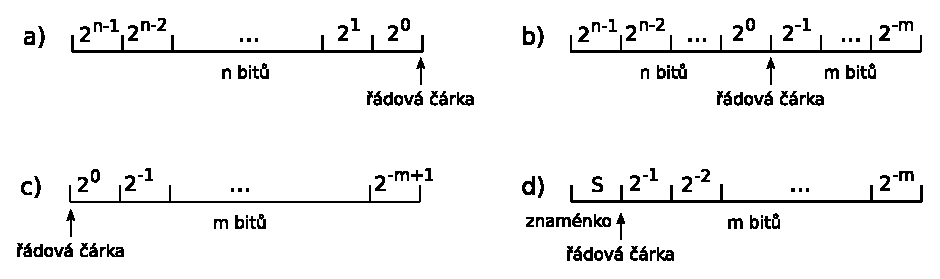
\includegraphics{obrazky/pevna_rad_carka.eps}}
\caption{Rôzne formáty fixed point aritmetiky \cite{KrausDisP}}
\label{formatfixpoint}
\end{figure}
\bigskip

%Môžme si všimnúť že čísla uložené vo FX sú rovnomerne rozložené na časovej ose.
Vo fixed point aritmetike sa používajú rôzne kódy, napr. priamy kód, doplnkový kód či inverzný kód. V~nasledujúcich kapitolách a pri návrhu integrátorov v~pevnej rádovej čiarke budeme používať doplnkový kód. 

\newpage
\section{Pohyblivá rádová čiarka}
Čísla uložené v~pohyblivej rádovej čiarke sú tvorené exponentom a mantisou. Všeobecný tvar na získanie hodnoty uloženej vo FP je nasledujúci:

\begin{eqnarray}
X = B^{E}\cdot M
\end{eqnarray}

\begin{tabular}{ll}
$ X $ - výsledná hodnota \\
$ B $ - základ sústavy \\
$ E $ - hodnota exponentu \\
$ M $ - mantisa \\
\end{tabular}
\bigskip

Zvýšením počtu bitov v~exponente $ E $ sa zvýši rozsah hodnôt, ktorý je možný reprezentovať, a zvýšením počtu bitov v~mantise $ M $ za zvýši presnosť uložených čísel. Existuje veľa formátov uloženia čísel v~pohyblivej rádovej čiarke. Najpoužívanejší a najrozšírenejší je štandard \textbf{IEEE 754}. Definuje vlastný formát uloženia čísel a viaceré formáty s~rôznou presnosťou. Najpoužívanejšie z~nich sú formáty čísel s~jednoduchou (single) a s~dvojitou (double) presnosťou. Čísla s~jednoduchou presnosťou sú uložené na 32 bitoch, kde MSB je znamienkový bit $ S $, ďalších 8 bitov tvorí exponent $ E $, a zvyšných 23 bitov tvorí mantisu $ M $.

\bigskip
\begin{figure}[h]
\centering
\scalebox{0.2}{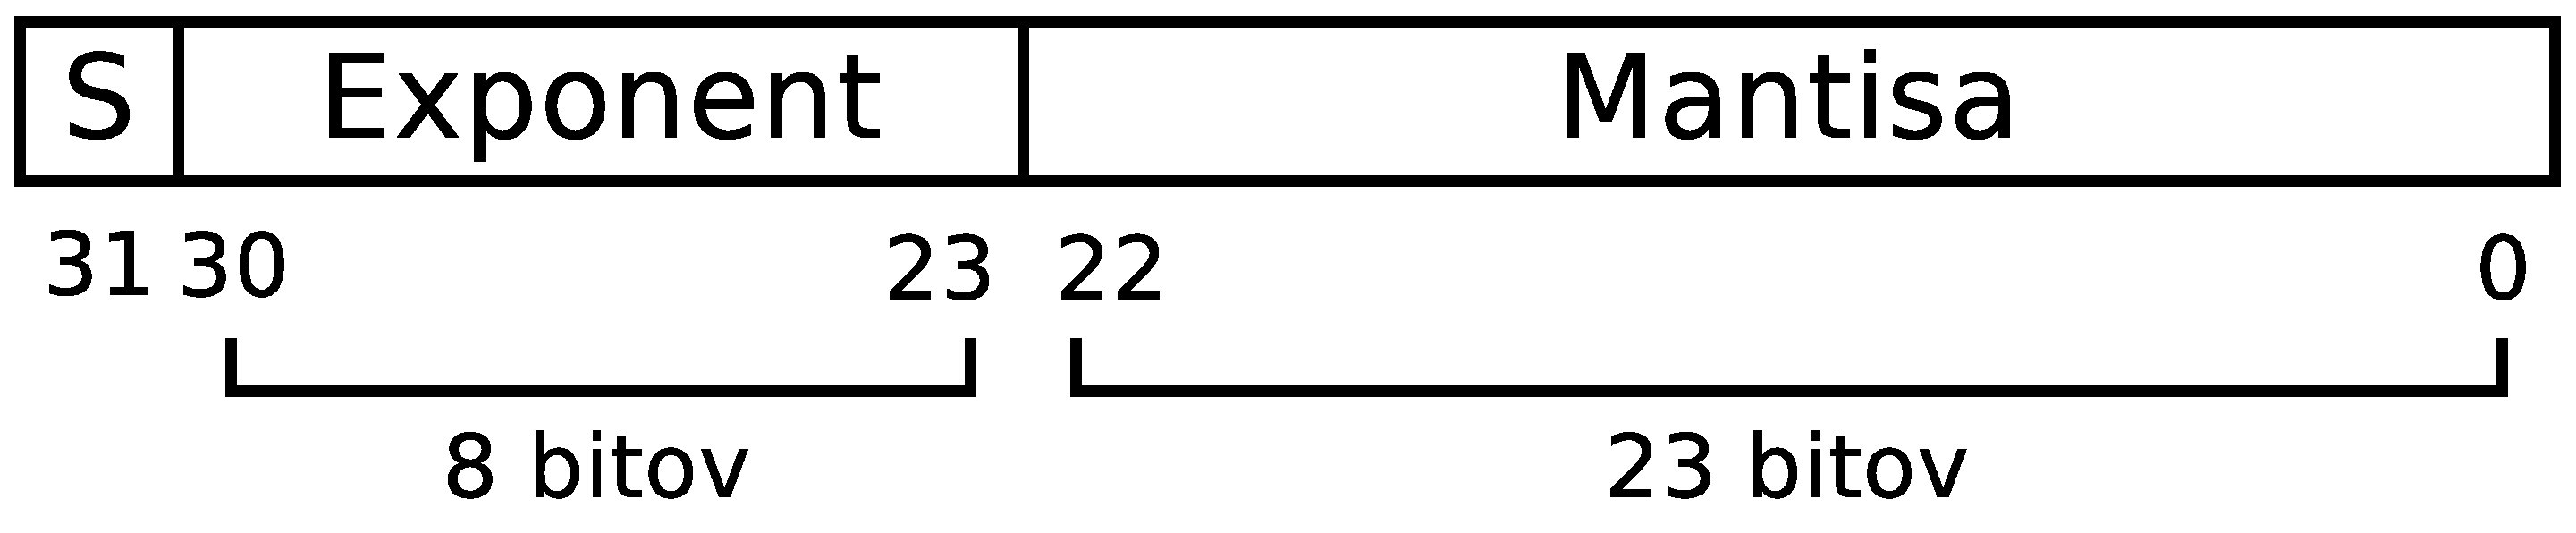
\includegraphics{obrazky/IEEE754_32b.eps}}
\caption{IEEE 754 formát s~jednoduchou presnosťou}
\label{formatFP32}
\end{figure}


Čísla s~dvojitou presnosťou sú uložené v~rovnakom formáte ako čísla s~jednoduchou presnosťou, avšak líšia sa v~počte bitov, ktorý je zväčšený na 64, kde MSB je znamienkový bit $ S $, ďalších 11 bitov tvorí exponent $ E $, a zvyšných 52 bitov tvorí mantisu $ M $.

\bigskip
\begin{figure}[h]
\centering
\scalebox{0.2}{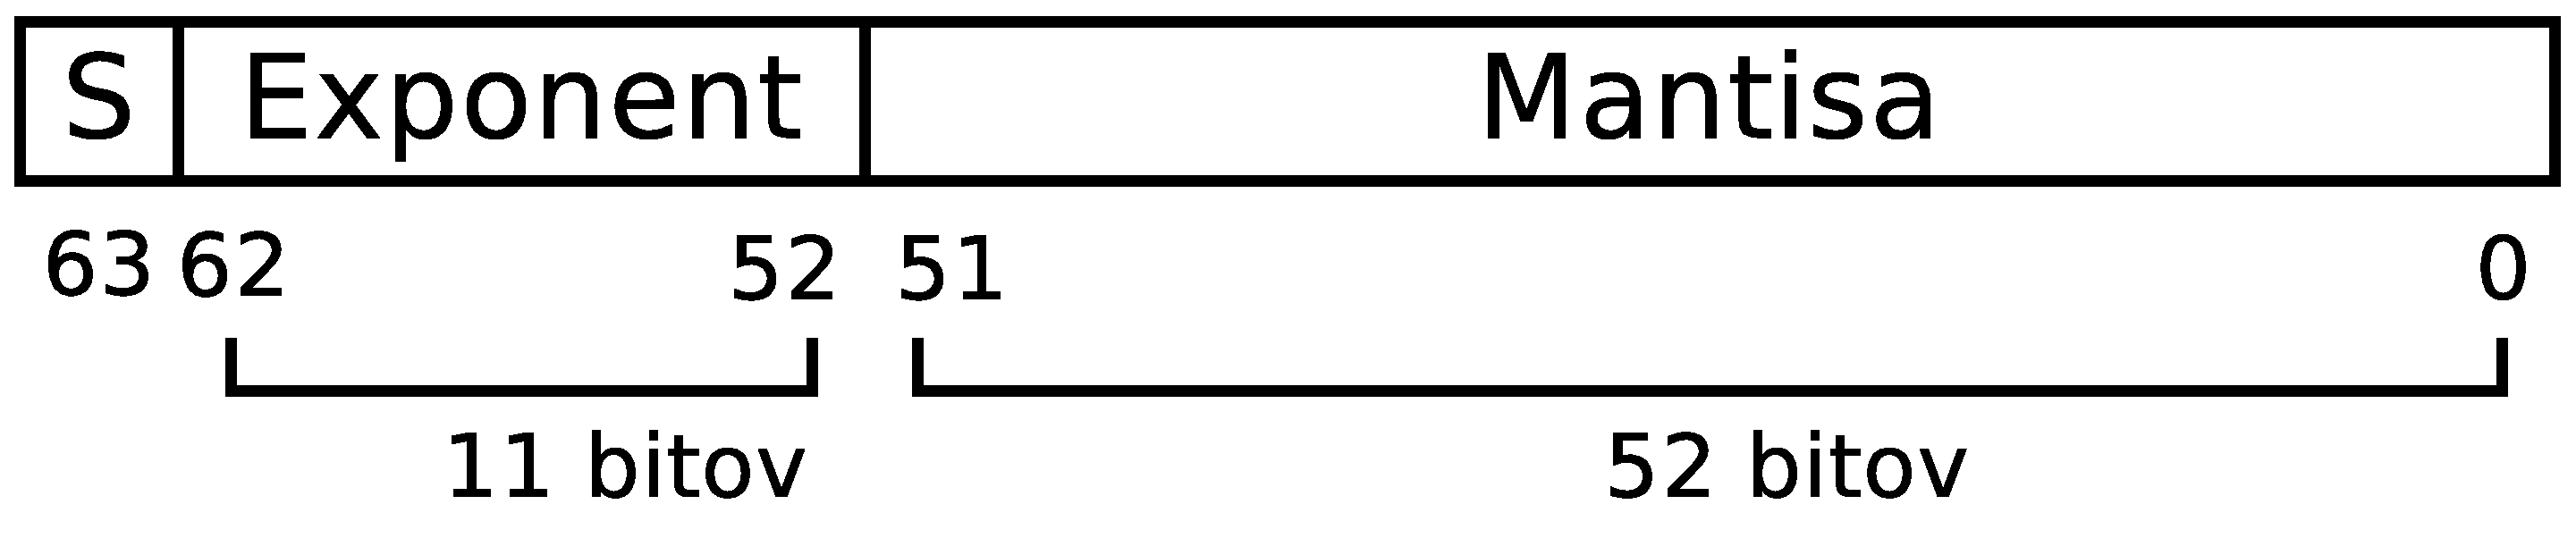
\includegraphics{obrazky/IEEE754_64b.eps}}
\caption{IEEE 754 formát s~dvojitou presnosťou}
\label{formatFP64}
\end{figure}

Znamienko $ S $ nadobúda hodnoty 0, čo značí kladné číslo; alebo 1, čo značí záporné číslo. Exponent je uložený v~kóde s~nepárnym posunutím o~hodnotu BIAS. Táto hodnota je zvolená tak, aby uložený exponent bol vždy kladný. Pri jednoduchej presnosti má teda BIAS hodnotu 127 a pri dvojitej presnosti hodnotu 2047.
\newpage
Hodnota mantisy je uložená v~priamom kóde bez znamienka, znížená o~hodnotu 1, keďže je tu použitá tzv. normalizácia. Mantisa je normalizovaná do tvaru $ 1.M $, kde sa jednotka neukladá -- je skrytá, čím sa ušetrí jeden bit. Hodnotu takto uloženého čísla získame zo vzťahu:

\begin{eqnarray}
X_{754} = -1^{S}\cdot 2^{E-BIAS}\cdot (1,M)
\end{eqnarray}

\begin{tabular}{ll}
$ X_{754} $ - výsledná hodnota \\
$ BIAS $ - 127 alebo 2047 \\
$ E $ - hodnota exponentu \\
$ M $ - mantisa \\
\end{tabular}
\bigskip

Štandard IEEE 754 definuje aj špeciálne hodnoty ako kladnú/zápornú nulu, kladné/záporné nekonečno, či hodnotu NaN (not a number). Tieto hodnoty sú uvedené v~tabuľke~\ref{standard_IEEE754}.
Hodnota mantisy v~normalizovanom tvare je v~intervale $ <1,0; 2,0) $. Ak tomu tak nie je, ide o~tzv. denormalizované číslo, a hodnota exponentu je braná ako $ -126 $. Štandard IEEE 754 definuje aj spôsob vykonávania základných matematických operácií, ktoré sú popísané v~sekciách \ref{PlusMinusFP} a \ref{MulDivFP}.

\bigskip
\begin{table}[h]
\centering
\begin{tabular}{|l|l|l|l|}
\hline
\rowcolor[HTML]{C0C0C0} 
S~(znamienko) & E (exponent) & M (mantisa)       & význam                    \\ \hline
0/1           & 00000000     & nulová hodnota    & +/- 0                     \\ \hline
0/1           & 00000000     & nenulová hodnota  & +/- denormalizované číslo \\ \hline
0/1           & 1 - 254      & ľubovoľná hodnota & +/- FP číslo              \\ \hline
0/1           & 11111111     & nulová hodnota    & +/- $ \infty  $           \\ \hline
0/1           & 11111111     & nenulová hodnota  & NaN                       \\ \hline
\end{tabular}
\caption{Štandard IEEE 754 \cite{FPOnline}}
\label{standard_IEEE754}
\end{table}

\newpage
\subsection{Súčet a rozdiel} \label{PlusMinusFP}
Súčet a rozdiel v~pohyblivej rádovej čiarke sa počíta podľa vzorcov
\begin{eqnarray}
X + Y = (M_{X}\cdot 2^{E_{X} - E_{Y}} + M_{Y})\cdot 2^{E_{Y}} \text{, kde} \quad E_{X} \leq E_{Y} \\
X - Y = (M_{X}\cdot 2^{E_{X} - E_{Y}} - M_{Y})\cdot 2^{E_{Y}} \text{, kde} \quad E_{X} \leq E_{Y}
\end{eqnarray}

Postup výpočtu operácie súčtu/rozdielu v~pohyblivej rádovej čiarke podľa štandardu IEEE 754 (\cite{FPOnline_operacie}, \cite{CamborBP}) je nasledovný:

\begin{enumerate}  
\item Na začiatku výpočtu sa obe čísla skontrolujú na výskyt špeciálnych hodnôt z~tabuľky~\ref{standard_IEEE754}. Ak ide o~špeciálne číslo, výsledok sa určí podľa tabuľky~\ref{special_plus}. Inak sa pokračuje bodom 2.

\item Vykoná sa porovnanie exponetov. Ak sú exponenty rozdielne, mantisu menšieho čísla posunieme o~rozdiel exponentov doprava. Tým docielime rovnosť oboch exponentov. Pri posune je dôležité, aby sme nezabudli na 1, ktorá je skrytá, kvôli normalizácií. Posun sa vykonáva spolu s~toutou 1. 

\item Následne sa porovnajú znamienka, a podľa výsledku sa vykoná sučet alebo rozdiel mantisy väčšieho čísla a posunutej mantisy. Ak došlo k~pretečeniu, mantisa výsledku sa posunie o~jeden bit doprava a hodnota exponentu sa zvýši. Aby bolo možné pretečenie detekovať, je potrebné sčítanie/odčítanie mantís vykonávať na sčítačke o~jeden bit väčšej než je veľkosť mantisy (veľkostou mantisy sa tu myslí počet bitov potrebných na uloženie mantisy aj so skrytou 1, čiže $ |1.M| + 1 $).

\item Ak je to potrebné, vykoná sa normalizácia. Mantisa sa posunie o~potrebný počet bitov doprava resp. doľava, tak, aby bola v~tvare $ 1.M $. O~daný počet bitov sa exponent zvýši resp. zníži.

\item Na koniec výpočtu sa skontroluje hodnota exponentu. Ak je hodnota maximálna, došlo k~pretečeniu výsledku. Ten sa nastaví podľa znamienka na kladné alebo záporné nekonečno. V~opačnom prípade, ak je hodnota exponentu minimálna (nulová), došlo k~podtečeniu, a výsledok je nastavený podľa znamienka na kladnú alebo zápornú nulu.
\end{enumerate}


\begin{table}[h]
\centering
\begin{tabular}{|l|l|l|}
\hline
\rowcolor[HTML]{C0C0C0} 
Hodnota operandu 1 & Hodnota operandu 2 & Výsledok sčítania \\ \hline
FP číslo           & +/- $ \infty $     & +/- $ \infty $    \\ \hline
+/- $ \infty $     & +/- $ \infty $     & +/- $ \infty $    \\ \hline
+ $ \infty $       & - $ \infty $       & NaN               \\ \hline
NaN                & ľubovoľná hodnota  & NaN               \\ \hline
\end{tabular}
\caption{Výsledok operácie sčítania so špeciálnymi hodnotami}
\label{special_plus}
\end{table}

\newpage
\subsection{Násobenie a delenie} \label{MulDivFP}
Násobenie a delenie v~pohyblivej rádovej čiarke sa počíta nasledovne:

\begin{eqnarray}
X \times Y = (M_{X} \cdot M_{Y})\cdot 2^{E_{X} + E_{Y}} \\
X \div Y = ({M_{X}} \div {M_{Y}})\cdot 2^{E_{X} - E_{Y}}
\end{eqnarray}

Postup výpočtu operácií násobenia a delenia podľa štandardu IEEE 754 (\cite{FPOnline_operacie}, \cite{CamborBP}) je nasledovný:

\begin{enumerate}  
\item Rovnako ako pri sčítaný, aj teraz sa na začiatku výpočtu skontroluje výskyt špeciálnych hodnôt oboch čísel podľa tabuľky~\ref{standard_IEEE754}. Ak ide o~špeciálne číslo, výsledok sa určí podľa tabuľky~\ref{special_nasobenie} alebo \ref{special_delenie}. Pri operácii delenia je potrebné kontrolovať nepovolenú operáciu delenie nulou. Pokračuje sa bodom 2.

\item Pri násobení sa hodnota exponentu vypočíta ako súčet exponentov, od ktorého sa odpočíta hodnota \textit{BIAS}. Pri operácii delenia sa hodnota exponentu vypočíta ako rozdiel exponentov, ku ktorému je pripočítaná hodnota \textit{BIAS}.

\item Výsledná mantisa je rovná sučinu resp. podielu mantís. Pri násobení je potrebné použiť násobičku, ktorej bitová šírka sa rovná dvojnásobku počtu bitov mantisy $ 1.M $. Ak dôjde k~pretečeniu alebo k~podtečeniu mantisy, vykoná sa posun mantisy doprava resp. doľava a hodnota exponentu sa zvýši resp. zníži.

\item Pokiaľ je to potrebné, prebehne normalizácia.

\item Na konci výpočtu sa skontroluje hodnota exponentu. Postupuje sa rovnako ako pri operácii súčtu: ak je hodnota exponentu maximálna, nastaví sa podľa znamienka na kladné alebo záporné nekonečno. V~opačnom prípade, ak je hodnota exponentu minimálna (nulová), výsledok sa nastaví podľa znamienka na kladnú alebo zápornú nulu.
\end{enumerate}


\begin{table}[h]
\centering
\begin{tabular}{|l|l|l|}
\hline
\rowcolor[HTML]{C0C0C0} 
Hodnota operandu 1 & Hodnota operandu 2 & Výsledok násobenia \\ \hline
kladné/záporné FP číslo & +/- $ \infty $ & +/- $ \infty $ \\ \hline
nula           & +/- $ \infty $ & NaN \\ \hline
+/- $ \infty $ & +/- $ \infty $ & +/- $ \infty $ \\ \hline
NaN & ľubovoľná hodnota & NaN \\ \hline
\end{tabular}
\caption{Výsledok operácie násobenia so špeciálnymi hodnotami}
\label{special_nasobenie}
\end{table}

\begin{table}[h]
\centering
\begin{tabular}{|l|l|l|}
\hline
\rowcolor[HTML]{C0C0C0} 
Hodnota operandu 1 & Hodnota operandu 2 & Výsledok násobenia \\ \hline
kladné/záporné FP číslo & +/- 0 & +/- $ \infty $ \\ \hline
0 & 0 & NaN \\ \hline
\end{tabular}
\caption{Výsledok operácie delenia so špeciálnymi hodnotami}
\label{special_delenie}
\end{table}

\chapter{Numerické integrátory} \label{NUM_INTEGRATORY}
Numerický integrátor je hardvérový komponent, ktorý slúži na výpočet numerickej integrácie. Podľa spôsobu výpočtu a komunikácie medzi komponentmi integrátora sa numerické integrátory delia na sériové, sériovo-paralelné a paralelné. My sa budeme zaoberať paralelnými numerickými integrátormi, kvôli ich jednoduchosti a rýchlosti výpočtu. V~nasledujúcich podkapitolách predstavíme jednotlivé návrhy paralelných násobiacich a paralelných deliacich integrátorov, oba typy v~pevnej a v~pohyblivej rádovej čiarke. Tieto integrátory obsahujú jeden vstup pre počiatočnú podmienku, dva vstupy pre prívod operandov a jeden výstup pre výsledok výpočtu. Schéma integrátora je znázornená na obrázku~\ref{schema_ndi}.


\begin{figure}[h]
\centering
\scalebox{0.6}{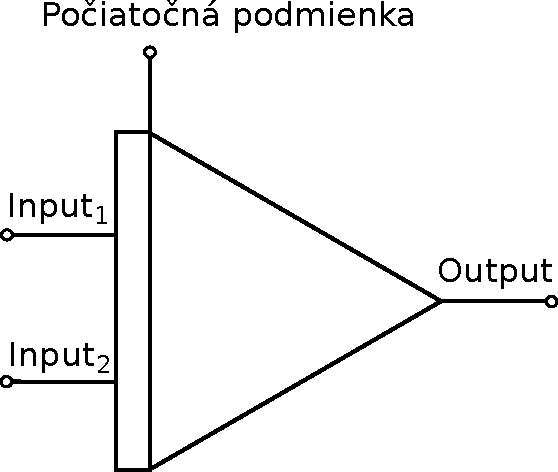
\includegraphics{obrazky/del_nas_integrator.pdf}}
\caption{Schéma násobiaceho/deliaceho integrátora}
\label{schema_ndi}
\end{figure}


\section{Násobiaci integrátor v~pevnej rádovej čiarke}
Násobiaci integrátor počíta rovnicu \eqref{dif_nasobenie} pomocou \eqref{DY1_cleny_nasobenia} -- \eqref{DY4_cleny_nasobenia}. Na základe týchto rovníc bol vytvorený návrh paralelného násobiacého integrátora, ktorý je na obrázku~\ref{ppni}. Návrh vychádza z~práce V. Závadu \cite{ZavadaBP} a bol upravený a rozšírený o~počet registrov $ DRn $ a $ DQn $, ktoré slúžia na ukladanie prichádzajúcich členov. Počet týchto registorov bol stanovený na 20. V~praxi sa používa podobný počet členov Tylorovej rady, ktorý vychádza z~toho, že poskytuje dobrý pomer medzi rýchlosťou a presnosťou.

Každý člen $ DYn $ obsahuje postupné delenie integračného kroku $ h $. Tieto hodnoty sú predpočítané a uložené v~sade registrov $ h $. Avšak nie je potrebné uložiť všetkých 20 hodnôt, stačí uložiť len tie hodnoty, ktorých deliteľ je nepárne číslo. Ostatné hodnoty je možné vypočítať jednoduchým posunom registra doprava, čo je vlastne delenie číslom 2. Týmto spôsobom znížime počet registrov o~polovicu. Počet operácií potrebných na výpočet sa nezvýši, keďže posun registra je možné vykonávať v~predstihu a paralelne s~inými operáciami.

\bigskip
\begin{figure}[h]
\centering
\scalebox{0.6}{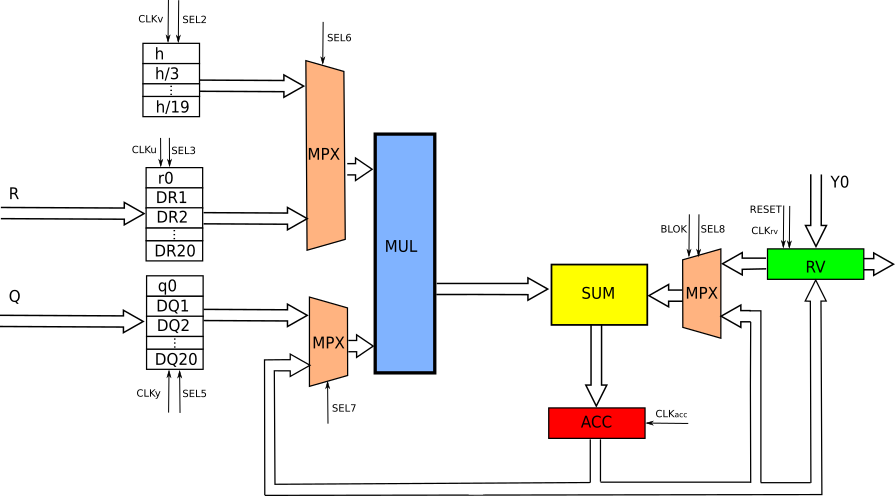
\includegraphics{obrazky/ppni_fx20.png}}
\caption{Paralelno-paralelný násobiaci integrátor \cite{ZavadaBP}}
\label{ppni}
\end{figure}

Na začiatku výpočtu sú pomocou signálu \textit{RESET} vynulované všetky registre, a nastavia sa potrebné signály na multiplexory \textit{MPX}. Následne je do registra \textit{RV} nahraná počiatočná podmienka, do registra \textit{h} je nahraný integračný krok metódy a do registrov \textit{h/i, i=3,5..19} sú nahrané predpočítané konštanty. Po prijatí hodnôt \textit{R} a \textit{Q} sa začne výpočet. Výsledok výpočtu je uložený v~registri \textit{RV}.


\section{Deliaci integrátor v~pevnej rádovej čiarke}
Tento integrátor počíta rovnicu \eqref{dif_delenie} pomocou členov \eqref{DY1_cleny_delenia} - \eqref{DY4_cleny_delenia}. Podobne, ako u~násobiaceho integrátora, bol z~týchto rovníc vytvorený návrh paralelného deliaceho integrátora. Návrh vychádza z~bakalárskej práce \cite{MatecnyBP} a bol upravený podobne ako predošlí násobiaci integrátor zvýšením počtu registrov $ DUn $ a $ DVn $. Taktiež sa zvýšil počet registrov $ DYn $, ktoré slúžia na uloženie jednotlivých členov Taylorovej rady. Deliaci integrátor, narozdiel od násobiaceho integrátora, nepoužíva sadu registrov $ h $, ale podobnú sadu registrov, ktorá obsahuje hodnoty $ 1/n $. Podobne ako u~násobiaceho integrátora je možné zmenšiť počet týchto registrov na polovicu s~využitím operácie \textit{shift}. Register \textit{const} obsahuje \textit{counter}, ktorý sa postupne inkrementuje, a s~ktorým sa násobí hodnota $ DYn $. Výsledná hodnota je uložená do daného registra $ DYn $ a znova použitá v~ďalšom výpočte, čím sa ušetrí operácia násobenia.

\begin{figure}[h]
\centering
\scalebox{0.5}{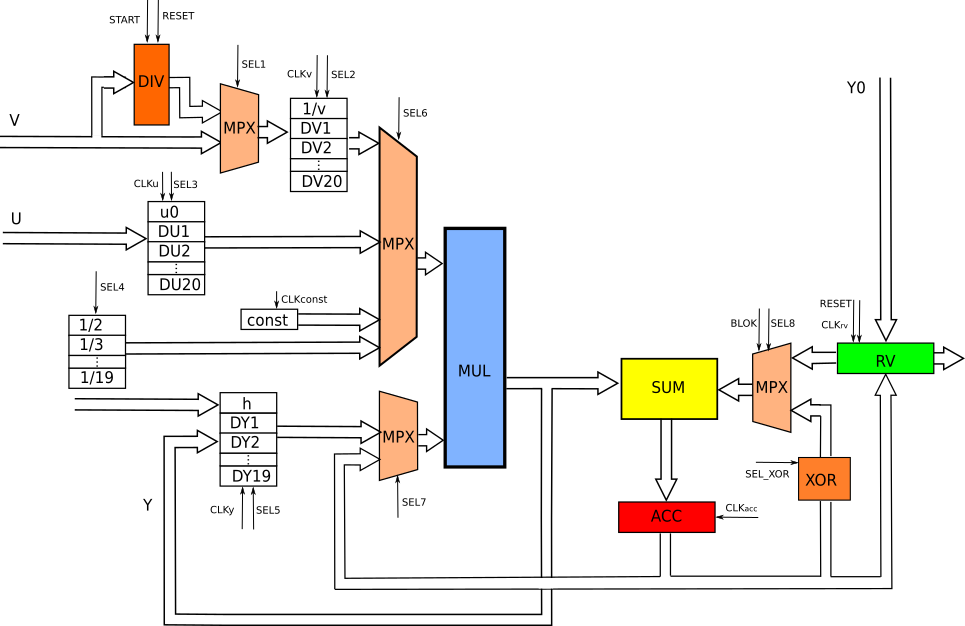
\includegraphics{obrazky/ppdi_fx20.png}}
\caption{Paralelno-paralelný deliaci integrátor \cite{MatecnyBP}}
\label{ppdi}
\end{figure}
\bigskip

\newpage
Podobne ako pri násobiacom integrátore, aj pri paralelnom deliacom integrátore sú na začiatku výpočtu vynulované registre pomocou signálu \textit{RESET} a nastavené signály multiplexorov \textit{MPX}. Ďalej je do registra \textit{RV} nahraná počiatočná podmienka a do registra $ h $ je nahraný integračný krok. Do registrov $ 1/n $ sú uložené predpočítané konštanty. Po prijatí hodnôt $ U $ a $ V $ sa začne výpočet. Hodnota $ V $ je privedená do deličky $ DIV $ a spustí sa výpočet $ 1/v $ s~použitím deliaceho algoritmu \textit{SRT}. Delenie je realizované len raz počas celého výpočtu, keďže ide o~veľmi náročnú operáciu. Kvôli optimalizácii je paralelne s~delením realizovaný výpočet násobenia $ uh $.
Po skončení výpočtu je výsledok uložený do registra $ RV $. 

\newpage
\section{Násobiaci integrátor v~pohyblivej rádovej čiarke}
Blokové schémy zapojenia integrátorov pracujúcich v~pohyblivej rádovej čiarke vychádzajú z~predchádzajúcich návrhov, ale boli rozšírené o~prácu so znamienkami, s~mantisou a s~exponentmi. Samotný výpočet exponenta sa deje v~komponente \textit{EXP}, ktorého návrh je zobrazený na obrázku~\ref{ppi_fp_exp}.

\bigskip
\begin{figure}[h]
\centering
\scalebox{0.8}{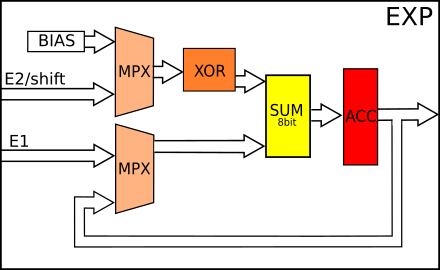
\includegraphics{obrazky/ppdi_fp_exp.png}}
\caption{EXP - blok pracujúci s~exponentmi}
\label{ppi_fp_exp}
\end{figure}
\bigskip

Komponent \textit{EXP} slúži na vykonávanie výpočtov s~exponentmi, ktoré sú popísané v~sekciách~\ref{PlusMinusFP} a~\ref{MulDivFP}. Obsahuje dva vstupy, do ktorých sú privedené jednotlivé exponenty z~komponentov $ DIV $, $ MUL $ a $ SUM $. Výpočet sa uskutočňuje pomocou paralelnej sčítačky na 8 alebo 11 bitoch, podľa v~závislosti použitej aritmetiky.
Pri vykonávaní operácie súčinu alebo rozdielu slúži komponent \textit{EXP} na výpočet rozdielu exponentov. Výsledná hodnota rozdielu je privedená naspäť do sčítačky \textit{SUM} cez register \textit{ACC}.
Pri operácii násobenia alebo delenia slúži komponent \textit{EXP} na výpočet výsledného exponentu. Podľa typu operácie sa vykoná sučet alebo rozdiel prijatých exponentov. Táto hodnota je uložená v~registri \textit{ACC} a privedená naspäť do sčítačky $ SUM_{8bit} $ s~hodnotou z~registra $ BIAS $. Vykoná sa súčet alebo rozdiel týchto hodnôt a výsledná hodnota je privedená naspäť do násobičky $ MUL $ alebo deličky $ DIV $.
Okrem spomenutých operácií slúži komponent $ EXP $ na zvýšenie alebo zníženie hodnoty exponenta na základe posunu mantisy pri pretečení/podtečení a pri normalizácii.

Kvôli prehľadnosti neobsahuje schéma zapojenia  znázornenie výpočtu znamienka a rozdelenie operandov na znamienko, exponent a na mantisu, a ich opätovné zloženie. Tieto oberácie sa vykonávajú v~komponentoch \textit{DIV}, \textit{MUL} a \textit{SUM}.\\

Návrh paraleného násobiaceho integrátora v~pohyblivej rádovej čiarke je na obrázku~\ref{ppni}. Čísla v~pohyblivej rádovej čiarke môžeme zobraziť presnejšie ako čísla v~pevnej rádovej čiarke, čiže pri uložení malých čísel v~pohyblivej rádovej čiarke dochádza k~menšej zaokrúhľovacej chybe. Z~tohto dôvodu je možné počítať Taylorovu radu s~použitím väčšieho počtu členov a zvýšiť tak presnoť výpočtu. Inegrátory v~pohyblivej rádovej čiarke sú teda navrhnuté tak, aby umožňovali výpočet až na 40 členov Taylorovej rady. Kvôli tomu, ako môžeme vidieť v~návrhu, je zvýšený počet registrov $ DRn $ a $ DQn $ na 40. Sada registrov $ h/i, i=3,5..39 $ obsahuje 20 registrov, kde sú zvyšné hodnoty dopočítané rovnako ako pri integrátoroch v~pevnej rádovej čiarke.

\begin{figure}[h]
\centering
\scalebox{0.6}{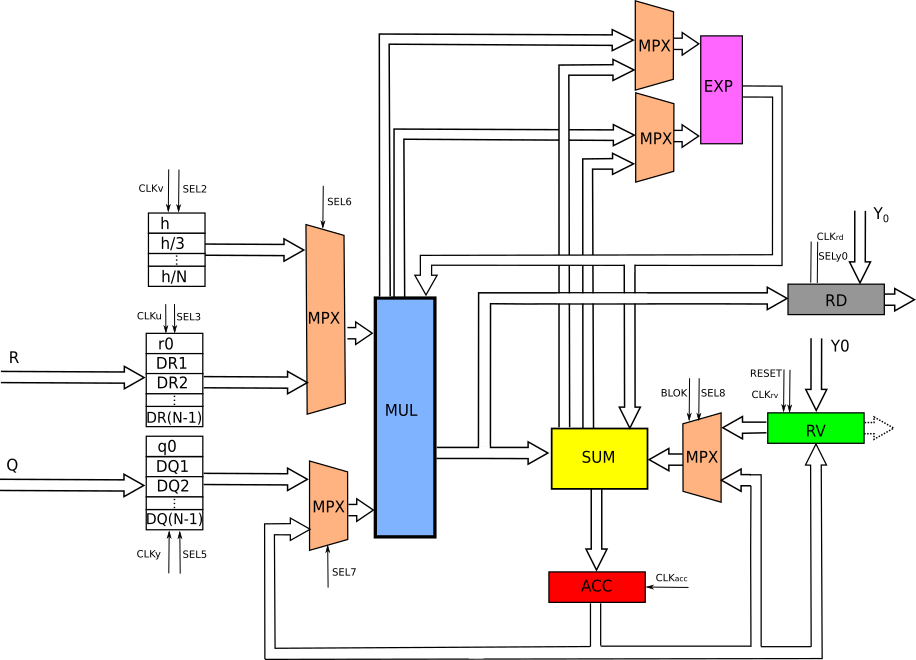
\includegraphics{obrazky/ppni_fp40.png}}
\caption{Paralelno-paralelný násobiaci integrátor v~pohyblivej rádovej čiarke}
\label{ppni_fp}
\end{figure}
\bigskip

Spôsob výpočtu paralelného násobiaceho integrátora v~pohyblivej rádovej čiarke je rovnaký ako pri násobiacom integrátore v~pevnej rádovej čiarke. Rozdielne sa vykonávajú operácie násobenia a sčítania. Po privedení hodnôt na vstupy násobičky $ MUL $ alebo sčítačky $ SUM $ sú čísla v~FP uložené do pomocných registrov v~týchto komponentoch. Z~týchto registrov sú jednotlivé časti FP čísla rozdistribuované do samostatných výpočetných obvodov. Znamienka sú privedené ku komponentu $ XOR $, ktorý vykonáva nonekvivalenciu. Exponenty, ako je popísané vyššie, spracúva komponent $ EXP $. Mantisy sú privedené do paralelnej násobičky alebo sčítačky. Výsledné hodnoty sú uložené do výstupného registra daného komponentu ($ MUL $ alebo $ SUM $) a poskytnuté na jeho výstupe k~ďalšiemu výpočtu.

\section{Deliaci integrátor v~pohyblivej rádovej čiarke}
Paralelný deliaci integrátor v~pohyblivej rádovej čiarke je najzložitejší z~navrhnutých integrátorov. Obsahuje všetky spomínané operácie: sčítanie, odčítanie, násobenie a delenie; a všetky vykonáva v~pohyblivej rádovej čiarke.
Operácie násobenia a sčítania sa vykonávajú rovnako ako v~paralelnom násobiacom integrátore v~pohyblivej rádovej čiarke. Operácia delenia sa vykonáva iba raz za celý výpočet a to paralelne s~operáciou násobenia, ako je tomu aj v~deliacom interátore v~FX aritmetikou. Tu však môže dôjsť ku kolízii v~použití komponentu $ EXP $. Keďže delenie je náročnou operáciou a jej vykonávanie je zdĺhavé, komponent $ EXP $ je poskytnutý najskôr na výpočet exponentov pri operácii násobenia. Po uvoľnení komponentu $ EXP $ násobičkou $ MUL $ je komponent $ EXP $ pridelený deličke $ DIV $ na výpočet exponentov. Po skončení delenia je podiel uložený do registra $ 1/v $ a pokračuje sa v~ďalšom výpočte.


\begin{figure}[h]
\centering
\scalebox{0.55}{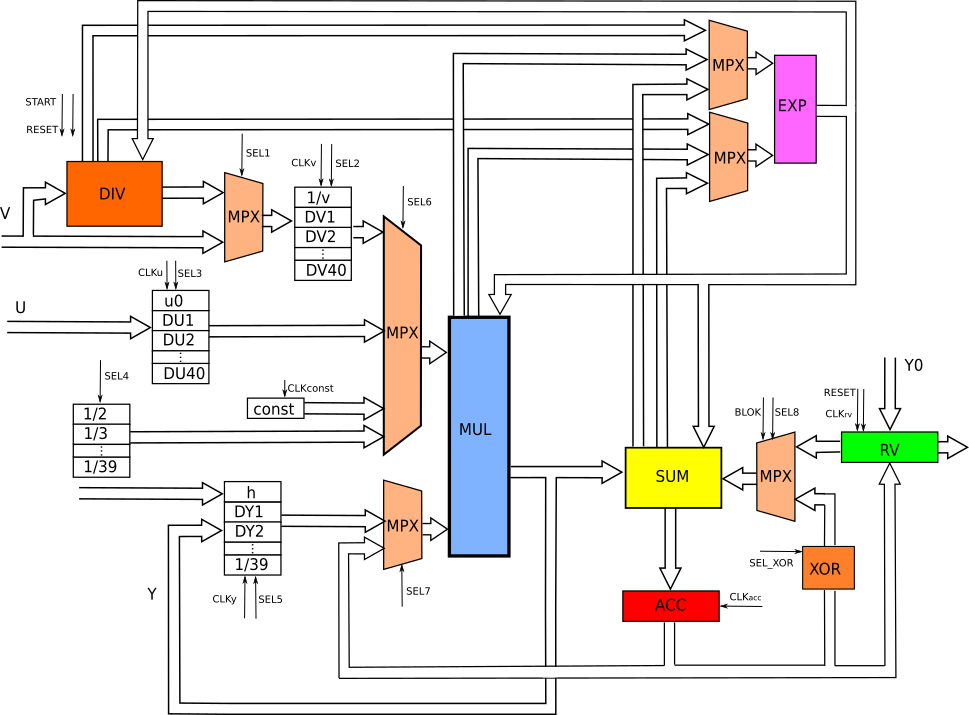
\includegraphics{obrazky/ppdi_fp40.png}}
\caption{Paralelno-paralelný deliaci integrátor v~pohyblivej rádovej čiarke}
\label{ppdi_fp}
\end{figure}
\bigskip


%\chapter{Implementácia integrátorv vo VHDL}
%\chapter{Analýza}
%\section{Porovanie Taylorovej rady s metódou Runge-Kutta 2. radu}
%\section{Porovanie Taylorovej rady s metódou Runge-Kutta 4. radu}

\chapter{Záver}
V~tejto práci sme sa zaoberali numerickou integráciou pomocou metódy Taylorovej rady. Úpravou jej členov sme získali potrebné rovnice, z~ktorých boli vytvorené jednotlivé návrhy integrátorov.
Rozšírili sme návrhy paralelných integrátorov s~operáciou násobenia a delenia v~pevnej rádovej čiarke tak, aby s~nimi bolo možné počítať diferenciálne rovnice na 20 členov Taylorovej rady. Ďalej sme tieto integrátory navrhli aj v~prevedení pohyblivej rádovej čiarky. Navrhli sme komponent slúžiaci na výpočet exponentu a na jeho úpravu pri normalizácii. Keďže výpočet v~aritmetike pohyblivej rádovej čiarky je presnejší, integrátory využívajúce túto aritmetiku sú navrhnuté na riešenie diferenciálnych rovníc až na 40 členov Taylorovej rady.

Ďalším pokračovaním práce je popísanie navrhnutých integrátorov vo VHDL, otestovanie ich funkčnosti na VIRTEX5 a následné analyzovanie ich časovej a priestorovej zložitosti v~porovnaní s~metódou Runge-Kutta.

%=========================================================================
